\documentclass[ ../main.tex]{subfiles}
\providecommand{\mainx}{..}

\newcommand{\ctor}[2]{\APFun{F}[#1][#2]}

\begin{document}
\section{Data types that model random approximate sets}
\label{sec:adt}
%A \emph{data structure} is a concrete representation of a data type. A popular implementation of \emph{random positive approximate sets} is the \emph{Bloom filter}.

%We call the set of axioms satisfied by a type and a set of functions on it a \emph{concept}.
%The \emph{concept} of the \emph{random approximate set} is given by the following set of axioms.


A \emph{data type} is a set and the elements of the set are called the \emph{values} of the data type.
We impose a \emph{structure} on sets (data types) by defining morphisms between them, such as operations like \emph{intersection} or relations like \emph{subset}.
Morphisms are also types.
Any data type needs one or more \emph{value constructors}, functions that map to values of the type.

%An \emph{abstract data type} is a set of objects whose behavior is defined by a set of values and a set of morphisms, where behavior is defined with respect to axiomatic semantics or operational semantics of an abstract machine.
%The abstract data type of the \emph{random approximate set} has an axiomatic specification.

The random approximate set is an abstract data type that models a \emph{set} with an additional set of \emph{probabilistic} axioms described in \cref{sec:asets}.
Suppose $T$ is a data type that overloads the \emph{member-of} predicate $\SetContains \colon \Set{U} \times T \mapsto \{0,1\}$ and has a \emph{value constructor} $\ctor{\fprate}{\tprate}$ that is a \emph{conditional probability distribution} over values of $T$ given elements of type $\PS{\Set{U}}$.
Data type $T$ \emph{models} the abstract data type of the random approximate set over elements in $\Set{U}$ with a false positive rate $\fprate$ and true positive rate $\tprate$ if \cref{asm:fprate,asm:tprate} are satisfied, i.e.,
\begin{equation}
	\Prob{\SetContains[x][\ctor{\fprate}{\tprate}(\Set{S})] \Given \SetNotContains[x][\Set{S}]} = \fprate
\end{equation}
and
\begin{equation}
	\Prob{\SetContains[x][\ctor{\fprate}{\tprate}(\Set{S})] \Given \SetContains[x][\Set{S}]} = \tprate\,.
\end{equation}
An instance of $T$ also models a classic set by its membership predicate, i.e., two sets are \emph{equal} if and only if they have the same members. We denote that an instance of $T$ models a set $\Set{A}$ by $T(\Set{A})$.

Normally, two different data types that model an abstract data type are \emph{exchangable} over a set of \emph{regular functions} without changing the result.
However, random approximate sets are \emph{probabilistic} so this strict definition of exchangability does not capture the intended meaning.
The random approximate set model is a \emph{frequentistic probability} model where an event's probability is defined as the \emph{limit} of its relative frequency in a large number of trials.
Thus, we relax the definition of exchangability and conclude that two data types that model random approximate sets (or any other probabilistic abstract data type) should produce the same \emph{limit} of the relative frequency of results in a large number of \emph{independent runs}.

An important distinction must be made with respect to \emph{independent runs}.
The most straightforward meaning is, given any set $\Set{A} \in \PS{\Set{U}}$, at the limit, repeated applications of $\ctor{\fprate}{\tprate}(\Set{A})$ generates a sample that converges in distribution to $\ASet{A}[\fprate][\tprate]$.
However, we also wish to allow for \emph{deterministic} value constructors.\footnote{Deterministic algorithms compatible with the random approximate set model are common but frequently have an auxiliary seed which indexes a particular approximation in a family.}

\subsection{Deterministic value constructors}
Value constructors compatible with the random approximate set model may come in many forms.
For example, in \cref{sec:bool_search} we demonstrate an approximation of Boolean search where Boolean queries are deterministically mapped to approximate result sets compatible with the random approximate set model.

%Suppose we have a value constructor $\ctor \colon \PS{\Set{U}} \mapsto T$ where $T$ models random approximate sets over $\PS{\Set{U}}$ with true and false positive rates $\tprate$ and $\fprate$ respectively.
%For instance, in \cref{sec:bool_search}, even if the Boolean search indexes are based on \emph{non-deterministic} value %constructors, the resulting \emph{approximate result sets} that queries map to are \emph{deterministic} given these search %indexes.

Suppose $\ctor{\fprate}{\fprate} \colon \PS{\Set{U}} \mapsto T$ (i.e., a deterministic total function) maps sets in $\PS{\Set{U}}$ to objects of type $T$ that model random approximate sets over the input.
Since $T$ models the abstract data type of the set, there is a unique bijection between $T$ and $\PS{\Set{{U}}}$, i.e., every value in $T$ models a specific subset of $\Set{U}$.
Thus, we may view $\ctor{\fprate}{\fprate}$ as a function $\ctor{\fprate}{\tprate} \colon \PS{\Set{U}} \mapsto \PS{\Set{U}}$ with an \emph{image}
\begin{equation}
\Image(\ctor{\fprate}{\tprate}) = \SetBuilder{\ctor{\fprate}{\tprate}(\Set{A})}{\Set{A} \in \PS{\Set{U}}} \subseteq \PS{\Set{U}}\,.
\end{equation}
Since the value constructor $\ctor{\fprate}{\tprate}$ may map multiple input sets to the same output set and some sets in the codomain may not be mapped to by any set in the domain, $\ctor{\fprate}{\tprate}$ is (possibly) a non-surjective, non-injective function.

%\subsection{Algebraic properties}
%The only thing we can say with certainty \emph{a priori}\footnote{A priori knowledge is independent of experience.} about the image of $\ctor{\fprate}{\tprate}$ is that its members are subsets of $\Set{U}$ and it contains the empty set $\EmptySet$ and universal set $\Set{U}$.


\begin{definition}
A $\sigma$-algebra is closed under countable unions, intersections, and complements.
\end{definition}
The image of $\ctor{\fprate}{\tprate}$ is not necessarily a $\sigma$-algebra.
However, the subsets of $\Set{U}$ that may be constructed by countable complements, unions, and intersections for elements of the image along with the empty set $\EmptySet$ and the universal set $\Set{U}$ is by definition a $\sigma$-algebra and is denoted by $\sigma(\ctor{\fprate}{\fprate})$.

Since $\sigma(\ctor{\fprate}{\fprate})$ is a set of sets closed under unions, intersections, and complements, it is a Boolean algebra defined by the six-tuple 
$\left(
    \sigma(\ctor{\fprate}{\fprate}), \cup, \cap, \SetComplement, \EmptySet,\Set{U}
\right)$,
e.g., set-theoretic operations over the above Boolean algebra are of the form
\begin{equation}
\sigma(\ctor{\fprate}{\fprate}) \mapsto \sigma(\ctor{\fprate'}{\fprate'})
\end{equation}
and
\begin{equation}
    \sigma(\ctor{\fprate}{\fprate}) \times \sigma(\ctor{\fprate}{\fprate}) \mapsto \sigma(\ctor{\fprate}{\fprate})\,.
\end{equation}
%Note that neither \emph{positive} nor \emph{negative} approximate sets are closed under complementation and thus are not Boolean algebras, but rather \emph{semi-rings} under unions and intersections.

Suppose we have two Boolean algebras,
$\left(
    \sigma(\ctor), \cup, \cap, \SetComplement, \EmptySet,\Set{U}
\right)$ and 
$\left(
    \sigma(\operatorname{g}), \cup, \cap, \SetComplement, \EmptySet,\Set{U}
\right)$,
where $\ctor{\fprate}{\tprate}$ and $\operatorname{g}$ are value constructors for approximate sets over $\PS{\Set{U}}$. Set-theoretic operations over both Boolean algebras is the Boolean algebra
$\left(
    \Sigma(\ctor{\fprate}{\tprate},\operatorname{g}), \cup, \cap, \SetComplement, \EmptySet,\Set{U}
\right)$
where $\Sigma(\ctor{\fprate}{\tprate},\operatorname{g}) = \sigma\!\left(\sigma(\ctor) \cup \sigma(\operatorname{g}\right)$.
Note that $\sigma(\ctor{\fprate}{\tprate}), \sigma(\operatorname{g}) 
    \subseteq \Sigma(\ctor{\fprate}{\tprate},\operatorname{g})$,
so $\Sigma(\operatorname{f_1}, \cdots, \operatorname{f_n})$ converges to $\PS{\Set{U}}$ as $n \to \infty$,
where $\operatorname{f_1},\ldots,\operatorname{f_n}$ are different mappings.

\begin{remark}
It is often trivial to implement a family of deterministic value constructors $\PS{\Set{U}} \mapsto T = \{\operatorname{f_1},\ldots,\operatorname{f_n}\}$ with distinct $\sigma$-algebras where $T$ models random approximate sets over $\PS{\Set{U}}$.
Additionally, assuming each time an approximate set is constructed, a ``random'' value constructor from $\PS{\Set{U}} \mapsto T$ is invoked, then repeated invocations on some set $\Set{A} \in \PS{\Set{U}}$ generates a frequency distribution of sets that converges to $\ASet{A}$ as $n \to \infty$, e.g., ``randomly'' seeding a Bloom filter's hash function.
\end{remark}

%In some cases, it may be important for each objective set to 
%%%have a unique approximate set. A quantity of $n$ 
%%%%deterministic algorithms will label at least 
%$n$ objective sets differently. Unfortunately, there is no 
%%%guarantee that we can 
%satisfy such a requirement.
%\begin{proof}
%We say that a mapping
%    $\operatorname{p} \colon \sigma(\ctor) 
%%%\mapsto 
%        \sigma(\operatorname{g})$
%is a homomorphism if for all $\Set{A},\Set{B} \in 
%%%\sigma(\ctor)$,
%\begin{align}
%    \operatorname{p}(\EmptySet) &= \EmptySet\,,\\
%    \operatorname{p}(\Set{U}) &= \Set{U}\,,\\
%    \operatorname{p}(\Set{A} \cup \Set{B}) &= 
%        \operatorname{p}(\Set{A}) \cup 
%%%\operatorname{p}(\Set{B})\,,\\
%    \operatorname{p}(\Set{A} \cap \Set{B}) &= 
%        \operatorname{p}(\Set{A}) \cap 
%%%\operatorname{p}(\Set{B})\,.
%\end{align}
%Consider two distinct $\sigma$-algebras 
%%%$\sigma(\ctor)$ and 
%$\sigma(\operatorname{g})$ for $\PS{\{0,1\}}$. Suppose 
%%%$\ctor(\{0\}) = \EmptySet$, 
%%%%$\ctor(\{0,1\}) = \{0,1\}$, 
%%%%%$\operatorname{g}(\{0\}) = \{0\}$, and 
%%%%%%$\operatorname{g}(\{0,1\}) = \{0,1\}$. Then, 
%%%%%%%$\ctor(\{0\} \cup \{1\}) = $.
%\end{proof}

%The probability that a particular set is in the 
%%%$\sigma$-algebra is given by the
%probabilistic model. We are not necessarily interested in 
%%%performing this 
%computation. In fact, we are also not interested in 
%assigning %probabilities to 
%the sets in the $\sigma$-algebra; it is not even clear what 
%%%this would mean. 
%Rather, we wish to explore the \emph{algebraic properties} 
%of the approximate set model over a deterministic algorithm.
% PRODUCT sigma-algebra, cartesian products generate product sigma-algebras. This is needed for approximate
% relations paper!
%
%Let {\displaystyle (X_{1},\Sigma _{1})} (X_{1},\Sigma _{1}) and {\displaystyle (X_{2},\Sigma _{2})} (X_{2},\Sigma _{2}) be two measurable spaces. The $\sigma$-algebra for the corresponding product space {\displaystyle X_{1}\times X_{2}} X_{1}\times X_{2} is called the product $\sigma$-algebra and is defined by
%{\displaystyle \Sigma _{1}\times \Sigma _{2}=\sigma (\{B_{1}\times B_{2}:B_{1}\in \Sigma _{1},B_{2}\in \Sigma %_{2}\}).} \Sigma _{1}\times \Sigma _{2}=\sigma (\{B_{1}\times B_{2}:B_{1}\in \Sigma _{1},B_{2}\in \Sigma %_{2}\}).
%$\operatorname{F} \colon [0,1] \times [0,1] \times \PowerSet{U} \mapsto \PowerSet{U}$
%For a given false positive and false negative rate, we may construct a function
%$\ctor \colon \PowerSet{U} \mapsto \PowerSet{U}$
%$\ctor(\Set{X} ; \fprate, \fnrate) = \operatorname{F}(\fprate,\fnrate,\Set{X})$

How do we reconcile a deterministic value constructor $\ctor{\fprate}{\tprate} \colon \PS{\Set{U}} \mapsto T$ with the \emph{probabilistic model}?
In this context, the notion of \emph{probability} quantifies our \emph{ignorance}:
\begin{enumerate}
\item Given a set $\Set{S}$, we do not have complete \emph{a priori} knowledge about the set the value constructor maps to.
The approximate set model only provides \emph{a priori} knowledge about the probability distribution $\ASet{S}$.
We acquire \emph{a posterior} knowledge\footnote{A posteriori knowledge is dependent on experience.} by observing $\ctor{\fprate}{\tprate}(\Set{S})$.

\item Given $T(\Set{S})$, we do not have complete \emph{a priori} knowledge about $\Set{S}$.
According to the probabilistic model, the only \emph{a priori} knowledge we have is given by the specified \emph{expected} false positive and false negative rates.

We may acquire \emph{a posteriori} knowledge by evaluating $\ctor{\fprate}{\tprate}(\Set{A})$ for each $\Set{A} \in \PS{\Set{U}}$ and remembering the sets that map to $T(\Set{S})$.\footnote{If the approximate set is the result of the union, intersection, and complement of two or more approximate sets, then we must consider the closure.}
However, since $\ctor{\fprate}{\tprate}$ is (possibly) non-injective, one or more sets may map to $T(\Set{S})$ and thus this process may not completely eliminate uncertainty.
Additionally, the domain $\PS{\Set{U}}$ has a cardinality $2^{\Card{\Set{U}}}$ and thus exhaustive searches are impractical to compute even for relatively small domains.\footnote{In the case of \emph{countably infinite} domains, it is not even theoretically possible.}
%However, we may still reduce our uncertainty by mapping some subset of interest.
\end{enumerate}

Suppose $\Set{U}$ is finite. The set of deterministic value constructors 
$\PS{\Set{U}} \mapsto \PS{\Set{U}}$ has a cardinality $(2^u)^(2^u)$, and in a 
sense they are all compatible with the random approximate set model.

For instance, a 
Bloom filter (positive approximate set) may have a family of 
hash function that, for a particular binary coding of the 
elements of a given universal set, maps \emph{every} element 
in the universal set to the same hash. Thus, for instance, no 
matter the objective set $\Set{X} \subseteq \Set{U}$, it will 
map to $\Set{U}$. The Bloom filter had a theoretically sound 
implementation, but only after empirical evidence was it 
discovered that it was not suitable. This is an extremely 
unlikely outcome in the case of large universal sets, but as 
the cardinality of the universal set decreases, the 
probability of such an outcome increases. Indeed, at 
$\Card{U} = 2$, the probability of this outcome is $?$.

Thus, \emph{a priori} knowledge, e.g., a theoretically sound 
algorithm, is not in practice sufficient (although for large 
universal sets, the probability is negligible). The 
suitability of an algorithm can only be determined by 
acquring \emph{a posterior} knowledge.

We could explore the space of functions in the family and 
only choose those which, on some sample of objective sets of 
interest, generates the desired expectations for the false 
positive and false negative rates with the desired variances. 
Most of them will if constructed in the right sort of way.


A family of functions that are compatible with the 
probabilistic model is given by observing a particular 
realization $\Set{X} = \ASet{S}$ and outputting 
$\Set{X}$ on subsequent inputs of $\Set{S}$, i.e., caching 
the output of a \emph{non-deterministic} process that 
conforms to the probabilistic model. This is essentially how 
well-known implementations like the Bloom filter work, where 
the pseudo-randomness comes from mechanical devices like hash 
functions that approximate random oracles.

The false positive rate of the approximate set corresponding 
to objective set $\Set{X}$ is given by
\begin{equation}
    \fprateob(\Set{X}) = \frac{1}{\n} \sum_{x \in \SetComplement[\Set{X}]} \SetIndicator{\ctor{\fprate}{\tprate}(\Set{X})}(x)\,,
\end{equation}
where $\n = \Card{\SetComplement[\Set{X}]}$.

Let $\Set{U}_p$ denote the set of objective sets with cardinality $\p$. The 
\emph{mean} false positive rate,
\begin{equation}
    \overline{\fprate} = \frac{1}{\Card{\Set{U}_p}}
        \sum_{\Set{X} \in \Set{U}_p} \fprateob(\Set{X})\,,
\end{equation}
is an unbiased estimator of $\fprate$ and the population variance
\begin{equation}
    s^2_\fprate = \frac{1}{\Card{\Set{U}_p}}
        \sum_{\Set{X} \in \Set{U}_p} \fprateob(\Set{X})\,,
\end{equation}
is an unbiased estimator of $\Var{\FPR_\n} = \fprate(1-\fprate)/\n$.
\begin{proof}
We imagine that the function $\ctor{\fprate}{\tprate}$ caches the output of a \emph{non-deterministic} process that conforms to the probabilistic model.
Thus, each time the function maps an objective set $\Set{X}$ of cardinality $\p$ to its approximation, the algorithm \emph{observes} a realization of 
$\FPR_\n = \fprateob$.
Thus,
\begin{align}
    \overline{\fprate}
        &= \frac{1}{\Card{\Set{U}_p}} 
            \sum_{\Set{X_i} \in \Set{U}_p} \fprateob(\Set{X_i})\\
        &= \frac{1}{\Card{\Set{U}_p}} 
            \sum_{\Set{X_i} \in \Set{U}_p} \Expect{\FPR_\n^{(i)}} = \fprate\,.
\end{align}
\end{proof}

\subsection{Space complexity}
\label{sec:space_comp}
If the finite cardinality of a universe is $u$ and the set is \emph{dense} (and the approximation is also dense, i.e., the false negative rate is relatively 
small), then
\begin{equation}
    \mathcal{O}(u) \; \si{bits}
\end{equation}
are needed to code the set, which is independent of $\p$, the false positive rate, and the false negative rate.

The lower-bound on the \emph{expected} space complexity of a data structure that models the \emph{random approximate set} where the elements are over a \emph{countably infinite} universe is given by the following postulate.
\begin{postulate}
\label{pst:approx_l_b}
The \emph{information-theoretic lower-bound}\index{information-theoretic lower-bound} of a data structure that implements the countably infinite \emph{random approximate set} abstract data type has an \emph{expected} bit length given by
\begin{equation}
    -\tprate \log_2 \fprate \; \si{bits \per element}\,,
\end{equation}
where $\fprate > 0$ is the false positive rate\index{false positive rate} and $\tprate$ is the true positive\index{true positive rate}.
\end{postulate}

The \emph{relative space efficiency}\index{relative space efficiency} of a data structure\index{data structure} $X$ to a data structure $Y$ is some value greater than $0$ and is given by the ratio of the bit length of $Y$ to the bit length of $X$,
\begin{equation}
    \RE(X,Y) = \frac{\BL(Y)}{\BL{X}}\,,
\end{equation}
where $\BL$ is the bit length function.
If $\RE(X,Y) < 1$, $X$ is less efficient than $Y$, if $\RE(X,Y) > 1$, $X$ is more efficient than $Y$, and if $\RE(X,Y) = 1$, $X$ and $Y$ are equally efficient.
The absolute space efficiency is given by the following definition.
\begin{definition}
The absolute space efficiency of a data structure $X$, denoted by \AbsoluteEfficiency{$X$}, is some value between $0$ and $1$ and is given by the ratio of the bit length of the theoretical lower-bound to the bit length of $X$,
\begin{equation}
    \AbsoluteEfficiency(X) = \frac{\theta}{\BL(X)}\,,
\end{equation}
where $\BL(X)$ denotes the bit length of $X$ and $\theta$ denotes the bit length of the information-theoretic lower-bound.
The closer $\AbsoluteEfficiency(X)$ is to $1$, the more space-efficient the data structure.
A data structure that obtains an efficiency of $1$ is \emph{optimal}.\footnote{Sometimes, a data structure may only obtain the information-theoretic lower-bound with respect to the limit of some parameter, in which case the data structure \emph{asymptotically} obtains the lower-bound with respect to said parameter, the number of positives $\p$ being the most obvious parameter.}
\end{definition}

The \emph{absolute} space efficiency of a data structure $X$ implementing a random approximate set of an objective set with $\p$ elements with a false positive rate $\fprate$ and true positive rate $\tprate$ is given by
\begin{equation}
    \AbsoluteEfficiency(X) = \frac{-\p \tprate \log_2 \fprate}{\BL(X)}\,.
\end{equation}

A well-known implementation of countably infinite \emph{positive approximate set} is the Bloom filter\cite{bf} which has an expected space complexity given 
by
\begin{equation}
    -\frac{1}{\ln 2} \log_2 \fprate \; \si{bits \per element}\,,
\end{equation}
thus the absolute efficiency of the Bloom filter is $\ln 2 \approx 0.69$.
A practical implementation of the \emph{positive random approximate set} is given by the \emph{Perfect Hash Filter}\cite{phf}, which compares favorably to the Bloom filter in may circumstances.\footnote{The \emph{Singular Hash Set}\cite{shs} is an example of a data structure that obtains optimality using \emph{brute-force} search, so it is not practical for even relatively small objective sets. However, its primary purpose is analytic tractability.}

In \cref{dummyref}, we claimed that the method of moments estimator for $\p$ of an objective set given a particular realization of a random approximation set is undefined for countably infinite universes.
Suppose we have a data structure $X$ that \emph{models} random approximate sets with an \emph{expected} space complexity proportional to $\p$, i.e., $\p \cdot \operatorname{b}(\tprate,\fprate)$ bits, where $\operatorname{b}$ is the expected bits per \emph{positive} element given a false positive rate $\fprate$ and true positive rate $\tprate$.
Then, given an object $x$ of type $X$, an estimator of $\p$ is
\begin{equation}
	\widehat{\p} = \frac{\BL(x)}{\operatorname{b}(\tprate,\fprate)}\,,
\end{equation}
were $\BL$ is the bit length function.
An expected \emph{upper-bound} on the cardinality is obtained by plugging in the information-theoretic lower-bound $\operatorname{b}(\tprate,\fprate) = -\tprate \log_2 \fprate$ bits per element.

\subsubsection{Space efficiency of \emph{unions} and \emph{differences}}
As a way to implement \emph{insertions} and \emph{deletions}, we consider the space efficiency of the set-theoretic operations of unions and differences of approximate sets.

Let $\Set{S}[1] = \{x_{j_1}, \ldots, x_{j_m}\}$ and suppose we wish to insert the elements $x_{k_1},\ldots,x_{k_p}$ into $\Set{S}[1]$. If $X_1$ is a mutable 
object, then an \emph{insertion} operator may be applied on $X_1$ for each 
$x_{k_i}$, $i=1,\ldots, p$.

Alternatively, if $X_1$ is immutable, then we may construct another object, 
$X_2$, that implements the set $\Set{S}[2] = \{x_{k_1},\ldots, x_{k_p}\}$, and 
then apply the union function,
\begin{equation}
    \SetUnion[X_1][X_2]\,.
\end{equation}
If we replace $X_1$ and $X_2$ by objects that implement \emph{positive 
approximate sets} of $\Set{S}[1]$ and $\Set{S}[2]$ respectively, then by 
\cref{dummyref}, the false positive rate of the resulting approximate set is 
$\fprateob_1 + \fprateob_2 - \fprateob_1 \fprateob_2$.

The space efficiency of this positive approximate set is given by the following 
theorem.
\begin{theorem}
\label{thm:union_space_complexity}
Given two countably infinite positive approximate sets $\PASet{S}[1]$ and 
$\PASet{S}[2]$ respectively with false positive rates $\fprateob_1$ and 
$\fprateob_2$, the approximate set $\SetUnion[\PASet{S}[1]][\PASet{S}[2]]$, 
which has an induced false positive rate 
    $\fprateob_1 + \fprateob_2 - \fprateob_1 \fprateob_2$,
has an expected upper-bound on its absolute efficiency given by
\begin{equation}
\label{eq:union_space_complexity}
    \AbsoluteEfficiency(\fprateob_1, \fprateob_2 \Given \alpha_1, \alpha_2) =
    \frac{
        \log_2\!\left(
        \fprateob_1 + \fprateob_2 - \fprateob_1 \fprateob_2
        \right)}
        {
            \alpha_1 \log_2 \fprateob_1 + \alpha_2 \log_2 \fprateob_2
        }\,,
\end{equation}
where
\begin{equation}
\label{eq:union_space_complexity_bounds}
\begin{split}
    0 &< \alpha_1 = \frac{\Card{\Set{S}[1]}}
        {\Card{\SetUnion[\Set{S}[1]][\Set{S}[2]]}} \leq 1\,,\\
    0 &< \alpha_2 = \frac{\Card{\Set{S}[2]}}
        {\Card{\SetUnion[\Set{S}[1]][\Set{S}[2]]}} \leq 1\,,\\
    1 &\leq \alpha_1 + \alpha_2\,.
\end{split}
\end{equation}
As $\fprateob_j \to 1$ or $\fprateob_j \to 0$ for $j=1,2$, or 
    $(\fprateob_1, \fprateob_2) \to (1,1)$, 
the absolute efficiency goes to $0$.
\footnote{As $(\fprateob_1,\fprateob_2) \to (0,0)$, the absolute efficiency 
depends on the path taken. In most cases, it goes to $0$.}
\end{theorem}
\begin{proof}
The proof comes in two parts. First, we prove \cref{eq:union_space_complexity}, 
and then we prove the bounds on $\alpha_1$ and $\alpha_2$ given by 
\cref{eq:union_space_complexity_bounds}.

Let $X$ and $Y$ denote optimally space-efficient data structures that 
respectively implement positive approximate sets $\PASet{S}[1]$ and 
$\PASet{S}[2]$ with false positive rates $\fprateob_1$ and $\fprateob_2$. By 
\cref{dummyref}, their union has an induced false positive rate given by
\begin{equation}
    \fprateob_1 + \fprateob_2 + \fprateob_1 \fprateob_2\,.
\end{equation}
The information-theoretic lower-bound of the approximate set of 
$\SetUnion[\Set{S}[1]][\Set{S}[2]]$ with the above false positive rate is given 
by
\begin{equation}
    -\Card{\SetUnion[\Set{S}[1]][\Set{S}[2]]}
        \log_2 \! \left(\fprateob_1 + \fprateob_2 +
        \fprateob_1 \fprateob_2\right) \; \si{bits}\,.
\end{equation}
Since we assume we only have $X$ and $Y$ and it is not possible to enumerate the 
elements in either, we must implement their union by storing and separately 
querying both $X$ and $Y$. Since $X$ and $Y$ are optimal, 
$\BL(X) = -\Card{\Set{S}[1]} \log_2 \fprateob_1$ and 
$\BL(Y) = -\Card{\Set{S}[2]} \log_2 \fprateob_2$. 
Making these substitutions yields an absolute efficiency ???
\begin{equation}
\label{eq:proof_union_ae}
    \AbsoluteEfficiency = \frac{\Card{\SetUnion[\Set{S}[1]][\Set{S}[2]]} \log_2 \! \left(\fprateob_1 + \fprateob_2 + \fprateob_1 \fprateob_2\right)}{\Card{\Set{S}[1]} \log_2 \fprateob_1 + \Card{\Set{S}[2]} \log_2 \fprateob_2}\,.
\end{equation}
Letting
\begin{equation}
    \alpha_1 = \frac{\Card{\Set{S}[1]}}{\Card{\SetUnion[\Set{S}[1]][\Set{S}[2]]}} \; \text{and} \; \alpha_2 = \frac{\Card{\Set{S}[2]}}{\Card{\SetUnion[\Set{S}[1]][\Set{S}[2]]}}\,,
\end{equation}
we may rewrite \cref{eq:proof_union_ae} as
\begin{equation*}
    \frac{
        \log_2\!\left(\fprateob_1 + \fprateob_2 - \fprateob_1 \fprateob_2\right)}
    {
        \alpha_1 \log_2 \fprateob_1 + \alpha_2 \log_2 \fprateob_2
    }\,.\tag{\ref{eq:union_space_complexity} revisited}
\end{equation*}

In the second part of the proof, we prove the bounds on $\alpha_1$ and $\alpha_2$ as given by \cref{eq:union_space_complexity_bounds}.
Both $\alpha_1$ and $\alpha_2$ must be non-negative since each is the ratio of two positive numbers (cardinalities). If $\Card{\Set{S}[1]} \ll \Card{\Set{S}[2]}$, then $\alpha_1 \approx 0$. If $\Set{S}[1] \supset \Set{S}[2]$, then $\alpha_1 = 1$. A similar argument holds for $\alpha_2$. Finally,
\begin{equation}
    \alpha_1 + \alpha_2 = \frac{\Card{\Set{S}[1]} + \Card{\Set{S}[2]}}{\Card{\SetUnion[\Set{S}[1]][\Set{S}[2]]}}
\end{equation}
has a minimum value by assuming that $\Set{S}[1]$ and $\Set{S}[2]$ are disjoint sets (i.e., their intersection is the empty set), in which case
\begin{equation}
    \alpha_1 + \alpha_2 = \frac{\Card{\Set{S}[1]} + \Card{\Set{S}[2]}}{\Card{\Set{S}[1]} + \Card{\Set{S}[2]}} = 1\,.
\end{equation}
\end{proof}
See \cref{dummyref} for a contour plot of the expected lower-bound as a function of $\fprateob_1$ and $\fprateob_2$. As $\fprateob_1 \to 0$ or $\fprateob_2 \to 0$, the efficiency goes to $0$.

The lower-bound on the efficiency of the union of approximate sets is given by the following corollary.
\begin{corollary}
Given two positive, non-enumerable approximate sets with false positive rates $\fprateob_1$ and $\fprateob_2$, their union is an approximate set that has an efficiency that is expected to be greater than the lower bound given by
\begin{equation}
    \min \AbsoluteEfficiency(\fprateob_1, \fprateob_2) = \frac{
        \log_2\!\left(\fprateob_1 + \fprateob_2 - \fprateob_1 \fprateob_2\right)}
    {
        \log_2 \fprateob_1 \fprateob_2
    }\,.
\end{equation}
\end{corollary}


\begin{corollary}
If $\fprate_1 = \fprate_2 = \fprate$, then the absolute efficiency is given by
\begin{equation}
\AbsoluteEfficiency(\fprateob \Given \alpha) = \left(1 + \frac{\log_2(2 - \fprateob)}{\log_2 \fprateob}\right)\left(1 - \frac{\alpha}{2}\right)\,,
\end{equation}
where
\begin{equation}
    0 \leq \alpha = \frac{\Card{\SetIntersection[\Set{S}[1]][\Set{S}[2]]}}{\Card{\SetUnion[\Set{S}[1]][\Set{S}[2]]}} \leq 1\,,
\end{equation}
which is a monotonically decreasing function with respect to $\fprate$ and $\alpha$ with limits given by $\lim_{\fprateob \to 0} \AbsoluteEfficiency(\fprate) = 1$ and $\lim_{\fprate \to 1} \AbsoluteEfficiency(\fprate) = 0$.
\end{corollary}
See \cref{fig:cor_union_same_fprate} for a graphic illustration.

\begin{figure}
\centering
\caption{Expected lower-bound on efficiency of the union of two approximate sets, neither of which can be enumerated.}
\begin{tikzpicture}
%\selectcolormodel{gray}
    \begin{axis}
    [
        xmax=.999,
        xmin=.001,
        ymax=.999,
        ymin=.001,
        zmin=0,
        xlabel={$\fprate_1$},
        ylabel={$\fprate_2$},
        zlabel={$\min \AbsoluteEfficiency(\fprate_1,\fprate_2)$},
        axis lines=left,
        ztick=\empty,
        xmode=log,
        ymode=log,
        log ticks with fixed point,
        minor tick style={draw=none}
    ]
    \addplot3[
        contour gnuplot={levels={0.1,0.2,0.3,0.4}},
        domain=.001:.999,
        y domain=.001:.999
    ] {log2(x + y - x * y) / log2(x * y)};
    \end{axis}
\end{tikzpicture}
\label{fig:cor_union_same_fprate}
\end{figure}

\begin{figure}
\centering
\caption{Expected lower-bound on efficiency of the union of two approximate sets with the same false positive rate $\fprate$, neither of which can be enumerated.}
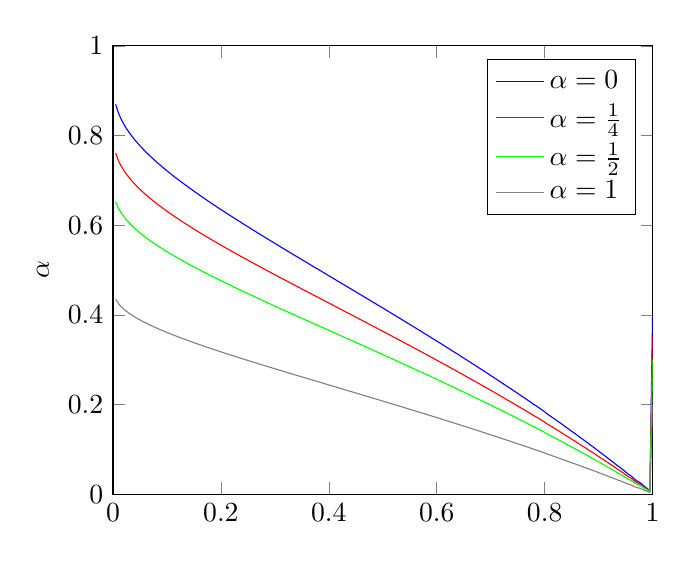
\begin{tikzpicture}
\begin{axis}
[
    xmax=1,
    xmin=0,
    ymax=1,
    ymin=0,
    xlabel={$\fprate$},
    ylabel={\AbsoluteEfficiency{$\fprate \Given \alpha$}},
    %no markers,
    %cycle list={black}
    legend style={nodes=right},
    legend pos={north east}
]
\addlegendentry{\AbsoluteEfficiency{$\fprate \Given \alpha=0$}}
\addplot[blue,domain=0:1,samples=200] {(1 + log2(2-x)/log2(x))};
\addlegendentry{\AbsoluteEfficiency{$\fprate \Given \alpha=\frac{1}{4}$}}
\addplot[red,domain=0:1,samples=200] {(1 + log2(2-x)/log2(x))*(.875)};
\addlegendentry{\AbsoluteEfficiency{$\fprate \Given \alpha=\frac{1}{2}$}}
\addplot[green,domain=0:1,samples=200] {(1 + log2(2-x)/log2(x))*(.75)};
\addlegendentry{\AbsoluteEfficiency{$\fprate \Given \alpha=1$}}
\addplot[gray,domain=0:1,samples=200] {(1 + log2(2-x)/log2(x))/2};
\end{axis}
\end{tikzpicture}
\label{fig:cor_union_same_fprate}
\end{figure}










\subsection{code tmp}

\subsection{Algebra of sets}
The perfect hash filter is a \emph{first-order} rate-distorted set, which is a type of \emph{random approximate set} whose error rates are due to rate-distortion.

Applying binary operators like \emph{union} or \emph{intersection} map pairs of first-order random approximate sets to \emph{second-order} random approximate sets.
If we continue in this trend, we generate higher-order random approximate sets, e.g., the union of a first-order set and a second-order set is a third-order set.

Note, however, that \emph{complements} of an $n$-th order set is an $n$-order set, i.e., the order of approximation is closed under complements.


When take the union of a pair of first-order random approximate sets, the result is a second-order set.


\begin{minted}{c++}
	template <
	FirstOrderApproximateSet A,
	FirstOrderApproximateSet B
	>
	struct second_order_approximate_set_union_expr
	{
		using value_type = A::value_type;
		
		auto contains(value_type x) { return a.contains(x) || b.contains(x); };
		A const a;
		B const b;	
	}
\end{minted}

\begin{minted}{c++}
	auto fpr(second_order_approximate_set_union_expr A)
	{
		// composed sets should be points. we decide to
		// span the points yielding a single interval.
		// TODO: should we move these to higher-order approximate set paper?
		return fpr(A.a)
	}
\end{minted}


\begin{minted}{c++}
	template <
	typename X,
	FirstOrderApproximateSet A,
	FirstOrderApproximateSet B
	>
	SecondOrderApproximateSetUnionExpr<X> operator+(A a, B b)
	{
		return SecondOrderApproximateSetUnionExpr<X>(a,b);
	}
\end{minted}


\begin{minted}{c++}
	template <
	typename X,
	FirstOrderApproximateSet A,
	FirstOrderApproximateSet B
	>
	SecondOrderApproximateSet<X> operator*(ApproximateSet<X> a, ApproximateSet<X> b)
	{
		return ~(~a + ~b);
	}
	
	
	
\end{minted}


Using type-erasure, we wrap arbitrarily complex expressions into \mintinline{c++}{ApproximateSet<X>}.
\begin{minted}{c++}
	template <
	typename X,
	FirstOrderApproximateSet A,
	FirstOrderApproximateSet B
	>
	ApproximateSet<X> operator*(ApproximateSet<X> a, ApproximateSet<X> b)
	{
		return ~(~a + ~b);
	}
\end{minted}





\end{document}
